% Options for packages loaded elsewhere
\PassOptionsToPackage{unicode}{hyperref}
\PassOptionsToPackage{hyphens}{url}
\PassOptionsToPackage{dvipsnames,svgnames,x11names}{xcolor}
%
\documentclass[
  11pt,
]{article}
\usepackage{amsmath,amssymb}
\usepackage{iftex}
\ifPDFTeX
  \usepackage[T1]{fontenc}
  \usepackage[utf8]{inputenc}
  \usepackage{textcomp} % provide euro and other symbols
\else % if luatex or xetex
  \usepackage{unicode-math} % this also loads fontspec
  \defaultfontfeatures{Scale=MatchLowercase}
  \defaultfontfeatures[\rmfamily]{Ligatures=TeX,Scale=1}
\fi
\usepackage{lmodern}
\ifPDFTeX\else
  % xetex/luatex font selection
\fi
% Use upquote if available, for straight quotes in verbatim environments
\IfFileExists{upquote.sty}{\usepackage{upquote}}{}
\IfFileExists{microtype.sty}{% use microtype if available
  \usepackage[]{microtype}
  \UseMicrotypeSet[protrusion]{basicmath} % disable protrusion for tt fonts
}{}
\makeatletter
\@ifundefined{KOMAClassName}{% if non-KOMA class
  \IfFileExists{parskip.sty}{%
    \usepackage{parskip}
  }{% else
    \setlength{\parindent}{0pt}
    \setlength{\parskip}{6pt plus 2pt minus 1pt}}
}{% if KOMA class
  \KOMAoptions{parskip=half}}
\makeatother
\usepackage{xcolor}
\usepackage[margin=25mm]{geometry}
\usepackage{longtable,booktabs,array}
\usepackage{calc} % for calculating minipage widths
% Correct order of tables after \paragraph or \subparagraph
\usepackage{etoolbox}
\makeatletter
\patchcmd\longtable{\par}{\if@noskipsec\mbox{}\fi\par}{}{}
\makeatother
% Allow footnotes in longtable head/foot
\IfFileExists{footnotehyper.sty}{\usepackage{footnotehyper}}{\usepackage{footnote}}
\makesavenoteenv{longtable}
\usepackage{graphicx}
\makeatletter
\def\maxwidth{\ifdim\Gin@nat@width>\linewidth\linewidth\else\Gin@nat@width\fi}
\def\maxheight{\ifdim\Gin@nat@height>\textheight\textheight\else\Gin@nat@height\fi}
\makeatother
% Scale images if necessary, so that they will not overflow the page
% margins by default, and it is still possible to overwrite the defaults
% using explicit options in \includegraphics[width, height, ...]{}
\setkeys{Gin}{width=\maxwidth,height=\maxheight,keepaspectratio}
% Set default figure placement to htbp
\makeatletter
\def\fps@figure{htbp}
\makeatother
\setlength{\emergencystretch}{3em} % prevent overfull lines
\providecommand{\tightlist}{%
  \setlength{\itemsep}{0pt}\setlength{\parskip}{0pt}}
\setcounter{secnumdepth}{5}
\newlength{\cslhangindent}
\setlength{\cslhangindent}{1.5em}
\newlength{\csllabelwidth}
\setlength{\csllabelwidth}{3em}
\newlength{\cslentryspacingunit} % times entry-spacing
\setlength{\cslentryspacingunit}{\parskip}
\newenvironment{CSLReferences}[2] % #1 hanging-ident, #2 entry spacing
 {% don't indent paragraphs
  \setlength{\parindent}{0pt}
  % turn on hanging indent if param 1 is 1
  \ifodd #1
  \let\oldpar\par
  \def\par{\hangindent=\cslhangindent\oldpar}
  \fi
  % set entry spacing
  \setlength{\parskip}{#2\cslentryspacingunit}
 }%
 {}
\usepackage{calc}
\newcommand{\CSLBlock}[1]{#1\hfill\break}
\newcommand{\CSLLeftMargin}[1]{\parbox[t]{\csllabelwidth}{#1}}
\newcommand{\CSLRightInline}[1]{\parbox[t]{\linewidth - \csllabelwidth}{#1}\break}
\newcommand{\CSLIndent}[1]{\hspace{\cslhangindent}#1}
\usepackage{microtype}
\usepackage{float}
\floatplacement{figure}{H}
\ifLuaTeX
  \usepackage{selnolig}  % disable illegal ligatures
\fi
\IfFileExists{bookmark.sty}{\usepackage{bookmark}}{\usepackage{hyperref}}
\IfFileExists{xurl.sty}{\usepackage{xurl}}{} % add URL line breaks if available
\urlstyle{same}
\hypersetup{
  pdftitle={Initialization and temporal-descriptor controls for quantum and classical compressed forecasting},
  colorlinks=true,
  linkcolor={Maroon},
  filecolor={Maroon},
  citecolor={Blue},
  urlcolor={teal},
  pdfcreator={LaTeX via pandoc}}

\title{Initialization and temporal-descriptor controls for quantum and
classical compressed forecasting}
\author{}
\date{Draft for author review, 10 October 2026}

\begin{document}
\maketitle

\hypertarget{abstract}{%
\section*{Abstract}\label{abstract}}
\addcontentsline{toc}{section}{Abstract}

Comparisons of quantum and classical compressed time-series models
depend on the information channel, initialization and evaluation
procedure. This study enforces fixed bottlenecks and common
feature-space scoring on bounded nonstationary synthetic sequences,
separates native decoder performance from linear readout of learned
representations and audits a candidate temporal-complexity criterion.
Exploratory paired controls identify a substantial
decoder-initialization effect: feature-neutral parameter centers lower
validation error in all 16 tested quantum pairs, with much of the
reduction already present before gradient training. A subsequently fixed
forecasting protocol evaluates eight fresh generator realizations, with
all model and probe selections hash-locked before test generation.
Reduced-rank regression has lower native forecast MSE than the quantum
transition encoder in all eight realizations; mean shifted-condition
errors are 0.091117 and 0.121666 respectively. The primary paired
difference is +0.030549 in favor of reduced-rank regression. An
exploratory nested analysis finds that adding validation descriptor
mismatch to model identity and validation forecast error raises held-out
squared prediction loss by 1.4\% and improves only 2 of eight
realization folds. Compensated orthogonal rotations change
coordinatewise descriptors while preserving probe predictions to
numerical precision. The evidence supports an initialization correction
and a reproducible small-scale negative benchmark for the tested
training procedure. It does not establish converged architecture
rankings, computational quantum advantage or an invariant
complexity-preservation principle.

\hypertarget{introduction}{%
\section{Introduction}\label{introduction}}

Compression is useful for prediction when a representation retains the
information required by the target. A representation's temporal
irregularity may offer a convenient diagnostic, but similarity between
input and latent complexity summaries is a separate claim from
preservation of predictive information. That distinction is especially
relevant when comparing classical coordinate compression with a quantum
subsystem: the state spaces, measurement channels and decoder
constraints differ.

Quantum autoencoders provide a framework for compressing quantum data
(\protect\hyperlink{ref-romero2017autoencoders}{Romero, Olson, and
Aspuru-Guzik 2017}). The present experiment instead embeds bounded
classical observations in a small quantum circuit and scores classical
prediction features. It therefore tests a particular hybrid
representation procedure rather than compression of arbitrary quantum
information. Benchmark design can strongly affect comparisons with
classical learning methods. Bowles, Ahmed and Schuld examine that issue
using diverse classification tasks and classical references
(\protect\hyperlink{ref-bowles2024benchmarking}{Bowles, Ahmed, and
Schuld 2024}). Their methodological concern motivates explicit baselines
and ablations here; their classification findings do not determine
forecasting performance in this study.

The corrected experiment addresses three questions. First, can a large
apparent quantum training deficit arise from the decoder's initial
readout after discarded qubits are reset? Second, does the corrected
quantum forecast procedure improve on a task-matched reduced-rank
predictor under controlled distribution shifts? Third, do
validation-only temporal descriptors add predictive value beyond
validation distortion and model identity when complete data realizations
are held out?

The contribution is a controlled evaluation and an accompanying
reproducibility record. It combines an initialization intervention with
matched initial encoders, a fresh-data forecasting comparison and a
separate exploratory regression analysis. It also demonstrates a
concrete coordinate dependence of the descriptor criterion. The
experiment is intentionally small and its conclusions concern the
implemented procedures within a fixed optimization budget.

\hypertarget{methods}{%
\section{Methods}\label{methods}}

\hypertarget{controlled-nonstationary-sequences}{%
\subsection{Controlled nonstationary
sequences}\label{controlled-nonstationary-sequences}}

Each realization uses an independently seeded four-by-two mixing matrix
with orthonormal columns. A two-dimensional Gaussian autoregressive
state evolves through three regimes, with boundaries after time points
41 and 84 in zero-based indexing. For each regime,

\[z_t=\rho_r z_{t-1}+(1-\rho_r)\mu_r+\sqrt{1-\rho_r^2}\,s_r\eta_t,
\qquad x_t=\tanh(Mz_t+\sigma\epsilon_t).\]

The innovations \(\eta_t\) and observation noise \(\epsilon_t\) are
independent standard Gaussian vectors. Regime means alternate sign and
have magnitudes proportional to \((0.5,1.0)\). The base mean-shift
amplitude is 0.15. The base state standard deviation is 0.35, multiplied
by 1.5 in the middle regime. Persistence is 0.35 in the outer regimes
and 0.75 in the middle regime; observation-noise standard deviation is
0.04. Innovation scaling fixes the within-regime stationary variance
when persistence changes. Regime transitions retain finite transients,
so the full sequence is nonstationary.

Each sequence contains 128 observations. Each realization supplies two
training sequences, two validation sequences and four test sequences per
condition. Independent random streams generate the partitions, sharing
the realization's mixing matrix. Models receive observation features,
not the generating states, mixing matrix or regime labels. Forecasting
uses 127 teacher-forced pairs per sequence: the observed input prefix
predicts its next observations. Evaluation does not roll predictions
forward as future inputs.

Test conditions include the base regime and five shifts. The mean shift
raises amplitude to 0.8. The variance shift raises the middle-regime
standard-deviation multiplier to 3, corresponding to a ninefold
middle-to-outer stationary variance ratio instead of 2.25. The
persistence shift uses -0.35 and 0.95. The noise shift uses
observation-noise standard deviation 0.25. The combined shift applies
all changes. These settings are controlled changes within one generator
family, not an exhaustive set of real-world shifts.

\hypertarget{enforced-compression-and-measurement}{%
\subsection{Enforced compression and
measurement}\label{enforced-compression-and-measurement}}

Classical ring encoders use Givens rotations. Their decoders receive the
first two retained coordinates and zeros in the two discarded positions.
This rotation-projection-rotation native map has two nonzero singular
values equal to one; it is more restricted than a general rank-two
forecast matrix with learned shrinkage. The quantum encoder embeds each
\(x_i\in[-1,1]\) as \(R_y(\arccos x_i)|0\rangle\), giving input \(Z\)
expectation \(x_i\). Its four-qubit encoder and decoder each use one
block. Each qubit has one shared angle applied in an \(R_x,R_y,R_z\)
sequence before and after a circular CZ layer. Four encoder and four
decoder angles give eight gradient-trained parameters. The no-CZ
ablation removes the entangling layers.

Quantum compression traces out the two fixed discarded qubits and
replaces them with \(|0\rangle\). It is implemented as a
trace-preserving density-matrix reset channel. Mixed retained states
remain mixed; the operation is not conditional postselection. Native
predictions are the four decoder \(Z\) expectations and are compared
directly with bounded observation targets. All quantum computation uses
exact classical density-matrix simulation, with no shot noise or quantum
hardware execution.

Common linear probes observe two retained coordinates from classical
encoders or two retained single-qubit \(Z\) expectations from quantum
encoders. The latter do not characterize the full reduced density
matrix. Equal readout dimension does not make the underlying quantum
state and classical representation equal in capacity.

Additional methods are a two-coordinate MLP encoder with hidden width
eight, a two-state GRU encoder with a width-eight feedforward decoder,
PCA, random orthogonal projection and reduced-rank regression. The GRU
reference supplies recurrent processing
(\protect\hyperlink{ref-cho2014encoder}{Cho et al. 2014}); the primary
quantum transition encoder is not recurrent. An uncompressed persistence
predictor retains all four coordinates. Untrained controls preserve the
seeded architecture and initialization of each gradient-trained method.
Zero-output and training-target-mean forecasts provide constant
references.

For reduced-rank regression, centered training inputs and next-time
targets define \(S_{xx}\) and \(S_{xy}\). The leading two singular
directions of \((S_{xx}+\lambda I)^{-1/2}S_{xy}\) define the encoder and
linear forecast decoder. Its native ridge penalty is selected on
validation from 0.001 and 0.01. PCA and random projection have native
reconstruction objectives; their native errors are excluded from
forecast comparisons and their forecasting capability is evaluated using
common probes.

\hypertarget{initialization-intervention}{%
\subsection{Initialization
intervention}\label{initialization-intervention}}

Near-zero quantum parameter jitter is uniform on \([-0.15,0.15]\).
Discarded qubits reset to \(|0\rangle\) have \(Z=1\), whereas discarded
classical coordinates are zero. A near-identity quantum decoder can
therefore start with a large output bias on discarded positions despite
small, centered observation features.

The feature-neutral initialization recenters only the existing
first-block decoder angles on discarded qubits. A bounded nonlinear
least-squares calibration minimizes their readouts for a synthetic
all-zero observation vector, holding the other seeded parameters fixed.
The center residual must be below \(10^{-8}\). The original seeded
jitter is then added to those centers, so the actual initialized
readouts need not be exactly zero. Calibration uses no training,
validation or test observations and adds no parameters or gates. Encoder
initialization is unchanged within each paired comparison.

The exploratory sensitivity grid uses previously inspected data seeds 17
and 41, initialization seeds 101 and 202, learning rates 0.02 and 0.08
and eight-epoch budgets on length-64 training and validation sequences.
No test partitions are generated in this grid. Only trajectories through
epoch eight are reused from an earlier sixteen-epoch control; its later
checkpoints are not represented as eight-epoch probe results.

\hypertarget{fresh-data-forecasting-protocol}{%
\subsection{Fresh-data forecasting
protocol}\label{fresh-data-forecasting-protocol}}

The protocol and runner were committed before fitting data seeds 113,
127, 139, 151, 163, 179, 191 and 211. Initialization seed 303 is fixed.
Feature-neutral initialization is used in both quantum variants. Every
gradient candidate completes eight epochs at each of two learning rates,
0.02 and 0.08. Native validation MSE selects the checkpoint and learning
rate. Quantum gradients use forward differences with width \(10^{-5}\)
and Adam; classical methods use automatic differentiation and Adam.
These are equal epoch budgets, not equal computation or a demonstration
of convergence.

For every selected and untrained representation, common ridge probes fit
training targets only. Validation selects penalties from 0.0001, 0.001
and 0.01. Native validation error selects encoder checkpoints
independently of probe scores. All 112 model/probe cases are fitted and
saved before any test partitions are generated. A selection lock hashes
251 configuration, data, checkpoint, probe and selection files. Test
evaluation accepts the frozen coefficients and verifies that these
hashes remain unchanged.

The primary endpoint averages native forecast MSE over the four
sequences in each shifted condition and then equally over the five
conditions. The prespecified contrast is quantum transition encoder
minus reduced-rank regression within each data realization. The eight
independently generated realizations are the replication units.
Individual sequences, conditions and models share a realization and are
not counted as independent evidence. No power or significance threshold
was specified.

\hypertarget{exploratory-descriptor-prediction}{%
\subsection{Exploratory descriptor
prediction}\label{exploratory-descriptor-prediction}}

Input and latent sequences are described by normalized order-three
permutation entropy, median-binarized LZ76 and lag-one correlation.
Permutation entropy summarizes ordinal patterns
(\protect\hyperlink{ref-bandt2002permutation}{Bandt and Pompe 2002}).
For each coordinate it is averaged over coarse-graining scales 1 and 2;
scale 4 is excluded because a 127-point prefix leaves fewer than 30
ordinal windows. LZ76 phrase count \(c(n)\) is scaled as
\(c(n)\log_2(n)/n\) for the binary alphabet
(\protect\hyperlink{ref-lempel1976complexity}{Lempel and Ziv 1976};
\protect\hyperlink{ref-vallat2026antropy}{Vallat 2026}). Finite-sample
values can exceed one. Constant-coordinate lag correlation is defined as
zero. Each summary is then averaged over coordinates.

The scalar mismatch is

\[d=\frac{1}{3}\left[(H_x-H_h)^2+(L_x-L_h)^2+
\left(\frac{r_x-r_h}{2}\right)^2\right].\]

This finite-sample descriptor distance is not an MDL codelength, a
sufficient statistic or an information-theoretic compression guarantee.
Research on latent generator complexity concerns a different objective
(\protect\hyperlink{ref-hu2023complexity}{Hu et al. 2023}).
Entropy-guided time-series classification is also an existing related
direction (\protect\hyperlink{ref-lin2026entrots}{Lin, Shen, and Wan
2026}). The present study audits a diagnostic association rather than
introducing entropy-based representation learning.

After inspection of the fresh-data forecast outcomes, an exploratory
analysis plan was committed before this regression analysis. Selected
checkpoints are restored without retraining and saved probes reproduce
validation errors. Descriptors are extracted only from the two
validation sequences, averaged over their 127-point input prefixes.
Validation features are saved and hashed before the analysis reads test
outcome rows. This ordering excludes test descriptors from the
predictors, but prior outcome inspection prevents a confirmatory
interpretation.

The primary regression target is common-probe forecast MSE averaged
across shifted conditions. Model identity and validation forecast-probe
MSE form the baseline. The primary extension adds scalar validation
mismatch. Model identity absorbs the fixed architecture and
training-budget differences among named procedures. Secondary extensions
use the three squared component mismatches or three latent descriptors.
Native forecasting and in-distribution probe error are secondary
targets. Native regressions exclude PCA and random projection and use
native validation forecasting error.

Nested leave-one-realization-out prediction withholds all models of each
outer data seed. On the remaining seven seeds, an inner
leave-one-realization-out loop selects ridge penalties from 0.001, 0.01,
0.1, 1 and 10. Centering, scaling and intercept estimation use fitting
rows only at both levels. Each outer loss is mean squared prediction
error on forecast MSE across that seed's models; eight outer losses
receive equal weight. There are 112 common-probe model/data cells but
only eight grouped prediction units. Every committed feature set is
reported without substituting a favorable secondary result for the
primary extension.

Finally, compensated orthogonal rotations transform latent coordinates
and adjust the linear probe accordingly. Predictions should remain
unchanged. Descriptor changes under this transformation, positive
scaling and time shuffling quantify coordinate sensitivity independently
of the prediction regression.

\hypertarget{results}{%
\section{Results}\label{results}}

\hypertarget{initial-output-bias-explains-a-substantial-optimization-deficit}{%
\subsection{Initial output bias explains a substantial optimization
deficit}\label{initial-output-bias-explains-a-substantial-optimization-deficit}}

Feature-neutral initialization reaches lower minimum validation MSE in
all 16 quantum pairs in the exploratory grid. The magnitude depends on
learning rate (Table 1). Raising the near-zero learning rate
substantially narrows the gap. Feature-neutral results vary less over
the two tested rates.

\begin{longtable}[]{@{}
  >{\raggedright\arraybackslash}p{(\columnwidth - 8\tabcolsep) * \real{0.1579}}
  >{\raggedleft\arraybackslash}p{(\columnwidth - 8\tabcolsep) * \real{0.2105}}
  >{\raggedleft\arraybackslash}p{(\columnwidth - 8\tabcolsep) * \real{0.2105}}
  >{\raggedleft\arraybackslash}p{(\columnwidth - 8\tabcolsep) * \real{0.2105}}
  >{\raggedleft\arraybackslash}p{(\columnwidth - 8\tabcolsep) * \real{0.2105}}@{}}
\toprule\noalign{}
\begin{minipage}[b]{\linewidth}\raggedright
Task
\end{minipage} & \begin{minipage}[b]{\linewidth}\raggedleft
Near-zero, 0.02
\end{minipage} & \begin{minipage}[b]{\linewidth}\raggedleft
Neutral, 0.02
\end{minipage} & \begin{minipage}[b]{\linewidth}\raggedleft
Near-zero, 0.08
\end{minipage} & \begin{minipage}[b]{\linewidth}\raggedleft
Neutral, 0.08
\end{minipage} \\
\midrule\noalign{}
\endhead
\bottomrule\noalign{}
\endlastfoot
Reconstruction & 0.440267 & 0.046814 & 0.108503 & 0.046727 \\
Forecast & 0.466011 & 0.071033 & 0.123432 & 0.067987 \\
\end{longtable}

Table 1. Native validation MSE, averaged over two data and two
initialization seeds for each learning rate. The four fits share two
data realizations and do not provide four independent data replicates.

Before gradient training, quantum reconstruction validation error drops
from 0.530160 to 0.049701 and forecasting error from 0.557219 to
0.075021 under the intervention. The zero-output forecasting reference
has validation error 0.072321. Thus a large paired improvement reflects
removal of a starting-output penalty; its size alone does not
demonstrate strong learned prediction. Paired encoder readout hashes and
initial probe errors match, isolating the changed decoder
initialization. These validation-only findings motivate the corrected
fresh-data procedure rather than a generalization claim.

\hypertarget{reduced-rank-regression-improves-the-prespecified-forecast-endpoint}{%
\subsection{Reduced-rank regression improves the prespecified forecast
endpoint}\label{reduced-rank-regression-improves-the-prespecified-forecast-endpoint}}

Mean shifted-test native forecast MSE is 0.121666 for the quantum
transition encoder and 0.091117 for reduced-rank regression. Quantum
minus reduced-rank differences are positive in all eight realizations,
with mean +0.030549 and observed range +0.014092 to +0.042249. Figure 1
shows every realization and the named native forecasting references. The
range is descriptive and is not a confidence interval.

\begin{figure}
\centering
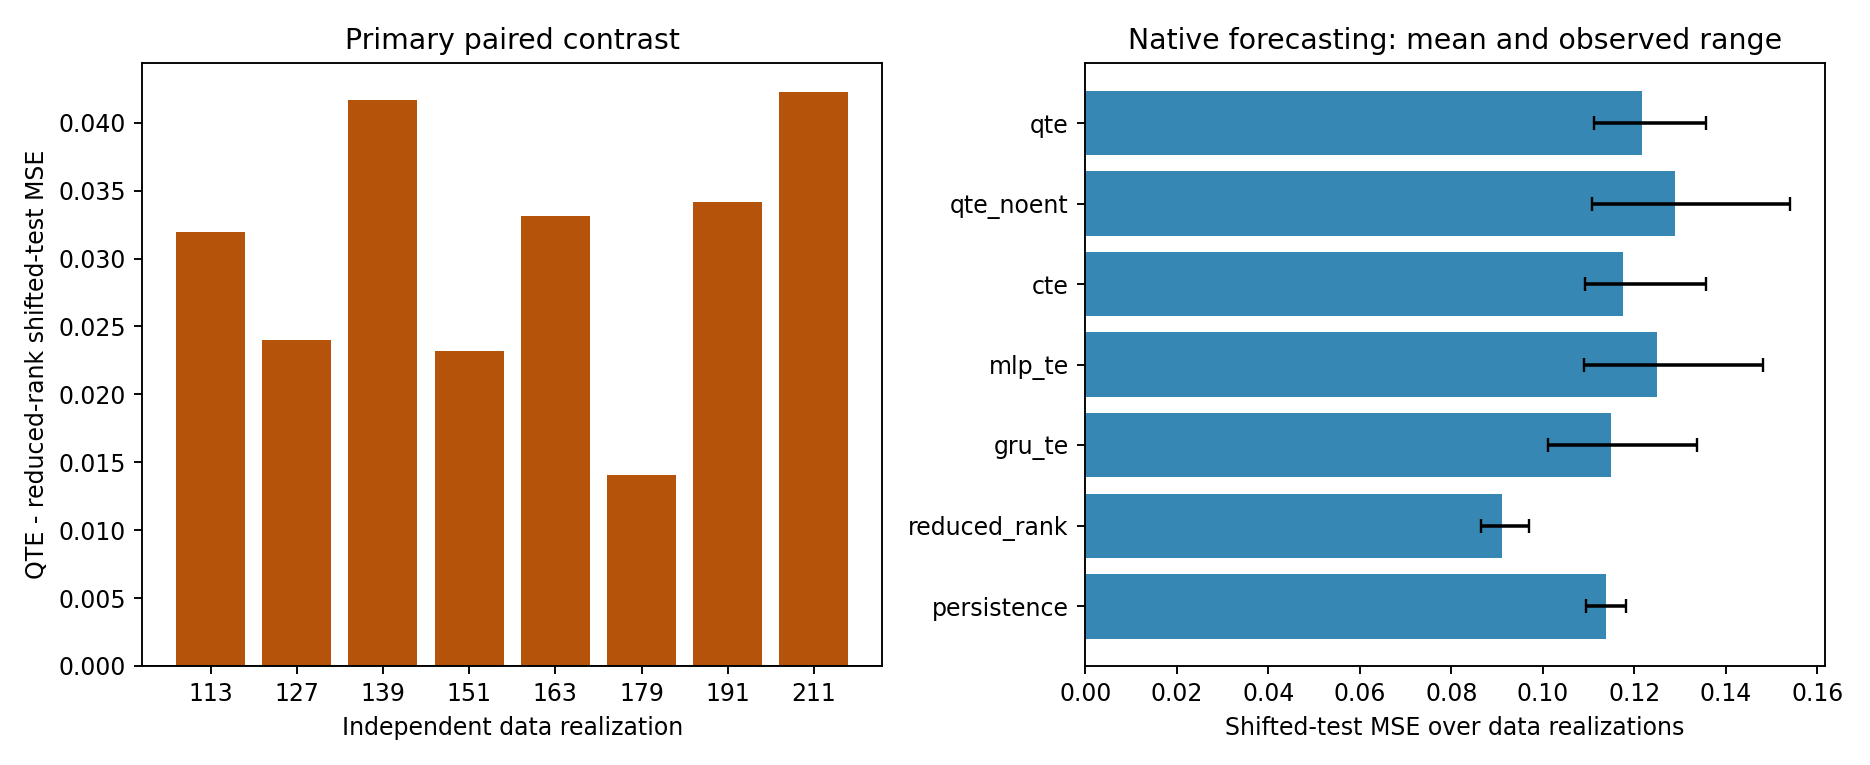
\includegraphics[width=1\textwidth,height=\textheight]{../docs/fresh_seed_forecasting/fresh_seed_forecasting.png}
\caption{Fresh-data primary contrast and native forecasting references.
Positive paired differences favor reduced-rank regression. Scores
average conditions equally within a realization. Error ranges show the
observed eight-realization range.}
\end{figure}

\begin{longtable}[]{@{}lrrr@{}}
\toprule\noalign{}
Model & Native ID & Native shifted & Probe shifted \\
\midrule\noalign{}
\endhead
\bottomrule\noalign{}
\endlastfoot
Quantum & 0.067188 & 0.121666 & 0.107755 \\
Quantum, no CZ & 0.074451 & 0.128927 & 0.108760 \\
Classical ring & 0.064519 & 0.117437 & 0.110042 \\
MLP & 0.070666 & 0.124979 & 0.098501 \\
GRU & 0.071634 & 0.114797 & 0.099974 \\
Reduced-rank & 0.054157 & 0.091117 & 0.090744 \\
Persistence & 0.068573 & 0.113704 & 0.091358 \\
Untrained quantum & 0.074516 & 0.131094 & 0.108299 \\
PCA & - & - & 0.089784 \\
\end{longtable}

Table 2. Means across the eight realizations. Persistence is an
uncompressed reference. PCA's native objective is reconstruction, so
only its forecast-probe score is shown. Common-probe decoder capacity is
shared, while representation and native decoder capacities differ.

The no-CZ native mean is 0.128927 and its common-probe mean is 0.108760.
Entanglement ablation therefore has different native and probe effects;
the experiment does not isolate a universal benefit from entanglement.
Reduced-rank regression has lower mean native error than the quantum
model in each named shifted condition. Persistence has the lowest mean
error in the mean-shift condition, emphasizing that aggregate ranking
depends on the chosen shift mixture.

The quantum common-probe shifted error is 0.107755 after training versus
0.108299 for its untrained control. Native errors are 0.121666 and
0.131094. The smaller probe change is consistent with much of the native
improvement occurring outside a large increase in linearly accessible
encoder usefulness. It does not identify a unique mechanism: checkpoint
selection uses native loss, the probe observes only two readouts and
optimization is limited to eight epochs.

\hypertarget{validation-descriptor-prediction-is-conditional-and-exploratory}{%
\subsection{Validation-descriptor prediction is conditional and
exploratory}\label{validation-descriptor-prediction-is-conditional-and-exploratory}}

The primary baseline has mean held-out squared prediction loss
\(7.353802\times10^{-5}\); adding scalar validation mismatch gives
\(7.455336\times10^{-5}\). The extension raises loss by 1.4\% and
improves 2/8 realization folds. The mean baseline-minus-extension
difference is \(-1.015344\times10^{-6}\), so its direction favors the
baseline. The squared component extension has loss
\(7.354606\times10^{-5}\), essentially unchanged from baseline, while
latent descriptors have loss \(7.957326\times10^{-5}\). These results
provide no positive primary evidence for incremental shifted-error
prediction from the chosen mismatch.

\begin{figure}
\centering
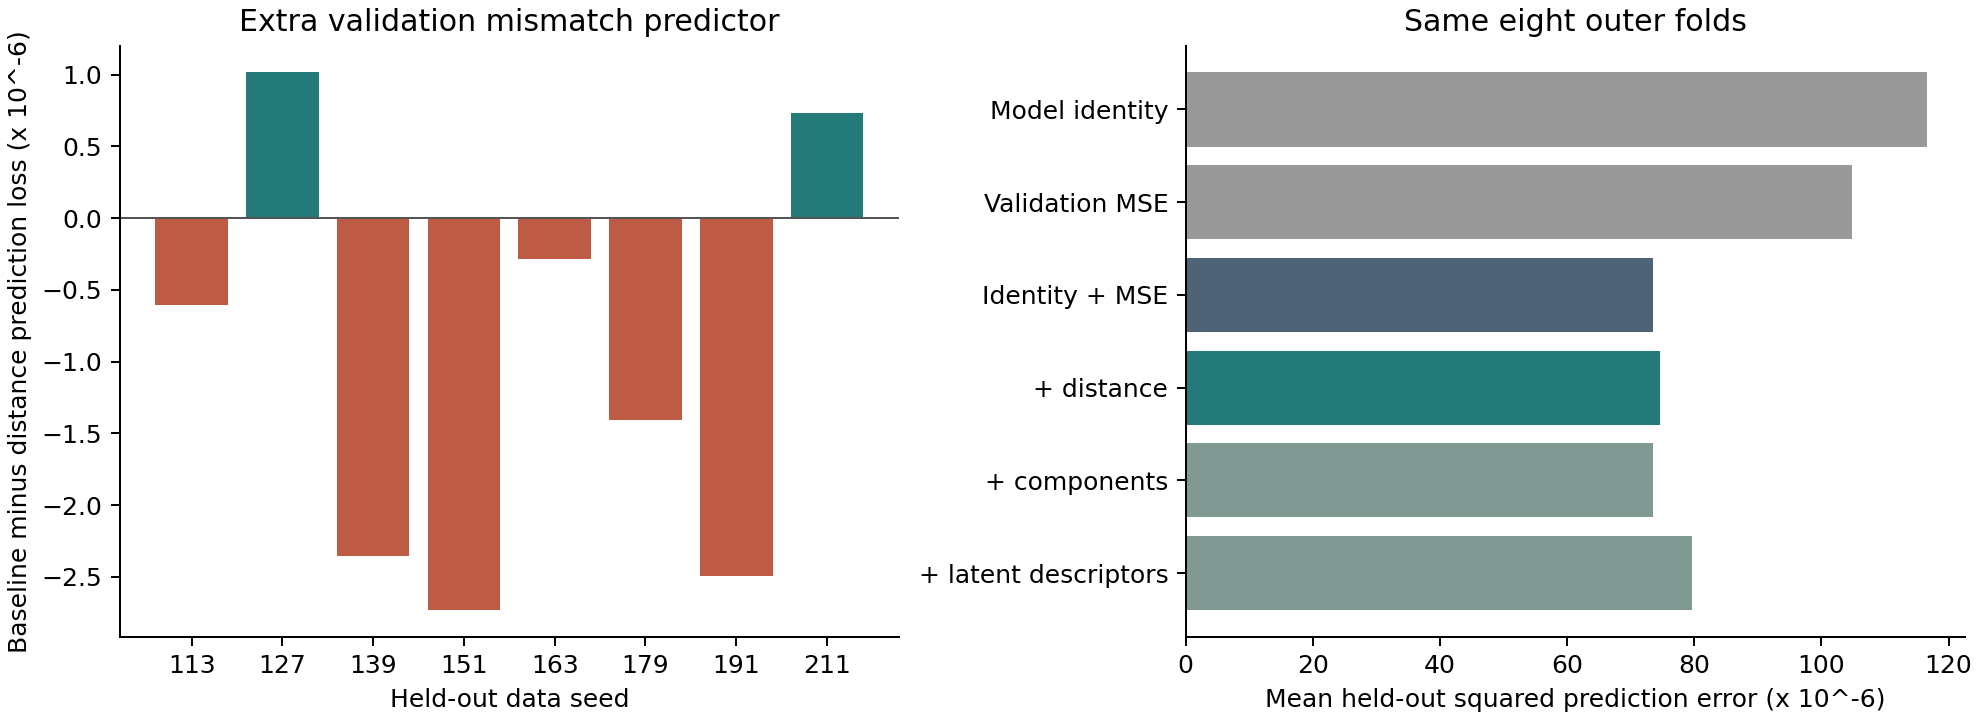
\includegraphics[width=1\textwidth,height=\textheight]{../docs/descriptor_generalization/descriptor_generalization.png}
\caption{Exploratory nested prediction of shifted common-probe forecast
MSE. Left: all eight baseline-minus-distance loss differences. Right:
all committed feature sets on the same outer folds. Loss units are MSE
squared.}
\end{figure}

\begin{longtable}[]{@{}lrrr@{}}
\toprule\noalign{}
Predictor & Shifted probe & ID probe & Shifted native \\
\midrule\noalign{}
\endhead
\bottomrule\noalign{}
\endlastfoot
Identity only & 11.667943 & 2.409838 & 14.835936 \\
Validation only & 10.477228 & 2.336336 & 14.399223 \\
Identity + validation & 7.353802 & 2.182675 & 11.697643 \\
+ distance (primary) & 7.455336 & 2.251772 & 12.261824 \\
+ components & 7.354606 & 2.280636 & 12.424297 \\
+ latent descriptors & 7.957326 & 2.104695 & 12.800469 \\
\end{longtable}

Table 3. Mean outer squared prediction losses in units of \(10^{-5}\)
MSE squared, across eight held-out realizations. Native forecasting
includes 12 cases per realization; common probes include 14. Secondary
feature sets and targets retain their exploratory status.

The results concern prediction across new realizations of this generator
with the same named model set. They do not evaluate prediction for
unseen architectures. Model identity alone and validation error alone
provide reference losses, while the controlled extension measures
incremental value beyond their joint baseline. Prior inspection, few
data realizations and a single initialization limit interpretation even
when an extension lowers grouped prediction loss.

\hypertarget{descriptor-distance-depends-on-coordinates}{%
\subsection{Descriptor distance depends on
coordinates}\label{descriptor-distance-depends-on-coordinates}}

Across existing forecast-task sequence rows, compensated rotations
change descriptor distance by a mean of 0.0019344 and a maximum of
0.0445319. Predictions differ by at most \(1.83\times10^{-15}\).
Positive scaling has maximum descriptor change \(1.03\times10^{-31}\);
time shuffling has mean descriptor change 0.0471076. The tiny scale and
prediction discrepancies reflect numerical precision.

For an orthogonal matrix \(R\), latent coordinates \(hR\) and
compensated coefficients \(R^TW\) satisfy \((hR)(R^TW)+b=hW+b\). The
prediction invariance follows algebraically; the recorded discrepancy
checks numerical implementation. Coordinatewise descriptor changes under
this equivalence demonstrate that matching the present summaries is not
a necessary invariant of linear predictive information. A different
multivariate or task-specific summary would require a new evaluation.

\hypertarget{computational-and-reproducibility-record}{%
\subsection{Computational and reproducibility
record}\label{computational-and-reproducibility-record}}

Quantum models use eight gradient-trained angles, the classical ring
uses eight parameters, the MLP uses 118 and the GRU uses 108. Analytic
methods have no gradient-trained parameters but have fitted coefficient
matrices. Mean fitting elapsed times per realization are 122.32 seconds
for the quantum model, 104.74 for no-CZ, 5.61 for the classical ring,
0.02 for the MLP and 0.24 for the GRU. Analytic fits take less than 0.01
seconds at this scale. These measurements include the implemented
selection procedures and concurrent CPU scheduling; they are not
hardware speedup estimates.

The fresh study fits with four independent CPU processes in 491.1
seconds and completes evaluation in 782.4 seconds. Its record contains
5,376 sequence/task metric rows and 384 constant-reference rows. All 251
locked files remain unchanged after evaluation. Saved observation and
generating-state arrays independently regenerate exactly. Compensated
rotation checks and finite diagnostics are recorded alongside source
hashes and package versions.

The descriptor follow-up restores all 112 saved cases and reproduces
locked validation-probe MSE with maximum absolute discrepancy
\(1.39\times10^{-17}\). Original selection files and validation-feature
hashes remain unchanged. All 1,920 held-out predictions are finite.
Regression tests verify checkpoint restoration for every model family
and the independence of outer-fold fitting from its held-out targets.

\hypertarget{discussion}{%
\section{Discussion}\label{discussion}}

The initialization intervention identifies an avoidable mismatch between
reset-qubit readout and zero-padded classical decoding. Its strongest
effect occurs before gradient training and its size changes with
learning rate. This supports reporting initial predictions, constant
baselines and matched untrained representations whenever low training
error is interpreted as learning. It also cautions against attributing
short-run quantum optimization failure directly to an intrinsic
training-landscape pathology.

In particular, flat loss histories or epoch-index curvature do not
establish a barren plateau. The relevant literature analyzes gradient
suppression and its scaling with system size under specified circuit
assumptions (\protect\hyperlink{ref-mcclean2018barren}{McClean et al.
2018}). This study uses four qubits and does not measure such scaling. A
decoder bias, optimization budget or unsuitable inductive bias can
explain poor finite-run performance without a barren-plateau conclusion.

The fresh-data comparison provides a negative result for the tested
quantum forecasting procedure against a low-rank classical predictor.
The generator has two Gaussian AR states mixed into four bounded
observations, making a linear low-rank reference especially relevant and
potentially favorable. That is a useful control for this task, not proof
that linear methods dominate on arbitrary nonlinear dynamics. The
reduced-rank comparison should be retained when exploring more difficult
generators, rather than replaced after observing its success.

Shared probes help separate decoder effects from representation
accessibility, but they cannot fully equate quantum and classical
capacity. A two-qubit reduced density matrix can encode structure not
captured by its two local \(Z\) expectations. Conversely, additional
observables would change measurement cost, feature dimension and the
evaluation protocol. The current result describes this restricted
readout and cannot be extended to the complete quantum state without
further work.

The descriptor analysis asks a more modest question than whether
complexity matching is essential: whether finite-sample validation
summaries improve prediction of error on another generator realization
after accounting for distortion and model identity. Nested grouped
validation gives that question a reproducible predictive test. It does
not erase prior outcome inspection. The rotation control adds a separate
mathematical reason to reject an invariant interpretation of the chosen
coordinatewise distance, regardless of whether it is useful as a
conditional empirical predictor.

The study has several material limits. Only one generator family and one
fresh-study initialization are evaluated. Two training sequences per
realization and an eight-epoch budget restrict conclusions about
convergence and optimization variability. Parameters, state spaces,
gradient estimators and computation differ across models. A GRU
comparison does not isolate the causal value of recurrence because the
architectures differ in other ways. The teacher-forced one-step task
does not address multi-step rollout, unknown forms of nonstationarity or
clinical/neuroimaging applicability. Eight exploratory descriptor folds
do not establish a general predictive law.

Further evidence should address these limits in a fixed extension:
multiple initialization seeds, stopping and convergence diagnostics
selected without test data, at least one substantially different
generator family and a genuinely untouched descriptor-prediction
replication. Such work could test the stability of the present
mechanisms and associations. It should keep task-matched simple
predictors, representation controls and resource accounting visible.

\hypertarget{code-and-data-availability}{%
\section{Code and data availability}\label{code-and-data-availability}}

Code, configurations, protocols, full sequence-level evidence and saved
checkpoint archives are maintained at
\url{https://github.com/TimeDelta/q-vs-c_enc_dec_nonstationary}. The
fresh-data protocol and selection lock precede test generation; the
descriptor protocol is explicitly exploratory after test inspection.
Reproduction commands and source identities appear in the respective
evidence reports. Original project material uses Zero-Clause BSD under
the repository's license scope. Imported material and dependencies
retain the notices recorded in the repository. The historical manuscript
is archived and its obsolete numerical conclusions are not used as
current evidence.

\hypertarget{references}{%
\section*{References}\label{references}}
\addcontentsline{toc}{section}{References}

\hypertarget{refs}{}
\begin{CSLReferences}{1}{0}
\leavevmode\vadjust pre{\hypertarget{ref-bandt2002permutation}{}}%
Bandt, Christoph, and Bernd Pompe. 2002. {``Permutation Entropy: A
Natural Complexity Measure for Time Series.''} \emph{Physical Review
Letters} 88: 174102.
\url{https://doi.org/10.1103/PhysRevLett.88.174102}.

\leavevmode\vadjust pre{\hypertarget{ref-bowles2024benchmarking}{}}%
Bowles, Joseph, Shahnawaz Ahmed, and Maria Schuld. 2024. {``Better Than
Classical? The Subtle Art of Benchmarking Quantum Machine Learning
Models.''} \url{https://doi.org/10.48550/arXiv.2403.07059}.

\leavevmode\vadjust pre{\hypertarget{ref-cho2014encoder}{}}%
Cho, Kyunghyun, Bart van Merrienboer, Caglar Gulcehre, Dzmitry Bahdanau,
Fethi Bougares, Holger Schwenk, and Yoshua Bengio. 2014. {``Learning
Phrase Representations Using {RNN} Encoder-Decoder for Statistical
Machine Translation.''} \url{https://arxiv.org/abs/1406.1078}.

\leavevmode\vadjust pre{\hypertarget{ref-hu2023complexity}{}}%
Hu, Tianyang, Fei Chen, Haonan Wang, Jiawei Li, Wenjia Wang, Jiacheng
Sun, and Zhenguo Li. 2023. {``Complexity Matters: Rethinking the Latent
Space for Generative Modeling.''}
\url{https://doi.org/10.48550/arXiv.2307.08283}.

\leavevmode\vadjust pre{\hypertarget{ref-lempel1976complexity}{}}%
Lempel, Abraham, and Jacob Ziv. 1976. {``On the Complexity of Finite
Sequences.''} \emph{IEEE Transactions on Information Theory} 22 (1):
75--81. \url{https://doi.org/10.1109/TIT.1976.1055501}.

\leavevmode\vadjust pre{\hypertarget{ref-lin2026entrots}{}}%
Lin, Guancen, Cong Shen, and Lin Wan. 2026. {``{EntroTS}: Entropy-Guided
Representation Learning for Time Series Classification.''} \emph{Chaos,
Solitons \& Fractals} 212: 119042.
\url{https://doi.org/10.1016/j.chaos.2026.119042}.

\leavevmode\vadjust pre{\hypertarget{ref-mcclean2018barren}{}}%
McClean, Jarrod R., Sergio Boixo, Vadim N. Smelyanskiy, Ryan Babbush,
and Hartmut Neven. 2018. {``Barren Plateaus in Quantum Neural Network
Training Landscapes.''} \emph{Nature Communications} 9: 4812.
\url{https://doi.org/10.1038/s41467-018-07090-4}.

\leavevmode\vadjust pre{\hypertarget{ref-romero2017autoencoders}{}}%
Romero, Jonathan, Jonathan P. Olson, and Alan Aspuru-Guzik. 2017.
{``Quantum Autoencoders for Efficient Compression of Quantum Data.''}
\emph{Quantum Science and Technology} 2 (4): 045001.
\url{https://doi.org/10.1088/2058-9565/aa8072}.

\leavevmode\vadjust pre{\hypertarget{ref-vallat2026antropy}{}}%
Vallat, Raphael. 2026. {``{AntroPy} 0.2.2: Entropy and Complexity of
Time Series in {Python}.''}
\url{https://raphaelvallat.com/antropy/generated/antropy.lziv_complexity.html}.

\end{CSLReferences}

\end{document}
